\documentclass[12pt, a4paper]{report}

\usepackage[utf8]{inputenc}
\usepackage[francais]{babel}
\usepackage{graphicx}
\usepackage{amsmath}
\usepackage{array}
\usepackage{gensymb}
\usepackage{eurosym}
\usepackage{siunitx}
\usepackage{colortbl}
\usepackage{tikz}
\usetikzlibrary{calc}

\usepackage[
    type={CC},
    modifier={by-nc-nd},
    version={4.0},
]{doclicense}

\usepackage[colorlinks=true,urlcolor=black,linkcolor=black]{hyperref}
\edef\UrlBreaks{\do\-\UrlBreaks}
\pdfpageattr {/Group << /S /Transparency /I true /CS /DeviceRGB>>} 

\newcommand*{\boxcolor}{orange}
\makeatletter
\renewcommand{\boxed}[1]{\textcolor{\boxcolor}{%
\tikz[baseline={([yshift=-1ex]current bounding box.center)}] \node [rectangle, minimum width=1ex,rounded corners,draw] {\normalcolor\m@th$\displaystyle#1$};}}
 \makeatother

\hyphenpenalty=10000
\renewcommand{\thesection}{\arabic{section}}
\newcommand*{\TakeFourierOrnament}[1]{{%
\fontencoding{U}\fontfamily{futs}\selectfont\char#1}}
\newcommand*{\danger}{\TakeFourierOrnament{66}}
\setlength\parindent{0pt}

\newcommand{\HRule}{\rule{\linewidth}{0.5mm}}
\newcommand{\gray}{\rowcolor[gray]{.90}}

\begin{document}
\renewcommand{\bibname}{Références}
\begin{center}
  
\includegraphics[scale=0.12]{textures/logo/heh_bw.pdf}

  \vspace{2cm}

  \textsc{\LARGE Projet ARS} \\ [0.5cm]
  \textsc{\Large Les différents systèmes d'exploitation} \\ [0.5cm]

  \textsc{\large 1er Bachelier en Informatique} \\ [0.2cm]
  \textsc{Groupe 5-8} \\

  \begingroup
  \fontfamily{pag} \selectfont 

  \HRule \\ [0.4cm] {
    \huge Architecture des Systèmes II \\ [0.2cm] 
  }
  (Laboratoire)
  \HRule \\ [1.3cm]
  \endgroup

  \begin{minipage}[t]{0.4 \textwidth} 
    \begin{flushleft} 
      \large \emph{Auteur:} \\ 
      Agozzino \textsc{Terencio} 
    \end{flushleft} 
  \end{minipage}
  % 
  \begin{minipage}[t]{0.4 \textwidth}
    \begin{flushright} 
      \large \emph{Auteur :} \\ 
      Ducobu \textsc{Alexandre} 
    \end{flushright} 
  \end{minipage}

  \vspace{0.5cm}

  \begin{minipage}[t]{0.4 \textwidth}
    \begin{center} 
      \large \emph{Enseignant:} \\ 
      Desmet \textsc{Erwin} 
    \end{center} 
  \end{minipage}

  \vspace{0.5cm}

  
\includegraphics[scale=0.08]{textures/logo/technical_bw.pdf}

  \vspace{0.5cm}

  Année académique 2015 - 2016
\end{center}

\thispagestyle{empty}

\newpage
\newpage
\thispagestyle{empty}
\setcounter{page}{0}
\null
\newpage
\newpage
\begin{center}
  
\includegraphics[scale=0.12]{textures/logo/heh.pdf}

  \vspace{2cm}

  \textsc{\LARGE Projet ARS} \\ [0.5cm]
  \textsc{\Large Les différents systèmes d'exploitation} \\ [0.5cm]

  \textsc{\large 1er Bachelier en Informatique} \\ [0.2cm]
  \textsc{Groupe 5-8} \\

  \begingroup
  \fontfamily{pag} \selectfont 

  \HRule \\ [0.4cm] {
    \huge Architecture des Systèmes II \\ [0.2cm] 
  }
  (Laboratoire)
  \HRule \\ [1.3cm]
  \endgroup

  \begin{minipage}[t]{0.4 \textwidth} 
    \begin{flushleft} 
      \large \emph{Auteur:} \\ 
      Agozzino \textsc{Terencio} 
    \end{flushleft} 
  \end{minipage}
  % 
  \begin{minipage}[t]{0.4 \textwidth}
    \begin{flushright} 
      \large \emph{Auteur :} \\ 
      Ducobu \textsc{Alexandre} 
    \end{flushright} 
  \end{minipage}

  \vspace{0.5cm}

  \begin{minipage}[t]{0.4 \textwidth}
    \begin{center} 
      \large \emph{Enseignant:} \\ 
      Desmet \textsc{Erwin} 
    \end{center} 
  \end{minipage}

  \vspace{0.5cm}

  
\includegraphics[scale=0.08]{textures/logo/technical.pdf}

  \vspace{0.5cm}

  Année académique 2015 - 2016
\end{center}

\thispagestyle{empty}

\newpage
\newpage
\thispagestyle{empty}
\setcounter{page}{0}
\null
\newpage
\newpage
\mbox{~}
\vfill
Ce document est mis à disposition selon les termes de la licence Creative
Commons ``\href{https://creativecommons.org/licenses/by-nc-nd/4.0/}{Attribution -
Pas d'utilisation commerciale 4.0 International}''.

\begin{figure}[!h]
  \centering
  
\includegraphics[width=0.25\textwidth]
  {textures/images/license/license.eps}
\end{figure}

\thispagestyle{empty}

\newpage
\tableofcontents
\newpage
\section{Introduction}
\subsection{Définition}
Tout ordinateur a besoin d'une sorte de « super-logiciel » qui se comporte
comme un chef d'orchestre afin de gérer l'utilisation des ressources
matérielles de l'ordinateur. \\ Ce super-logiciel porte un nom : système
d'exploitation (\textit{Operating System}). De nos jours, on en retrouve dans
la majorité des appareils électroniques (\textit{appareils photo numériques,
smartphones, serveurs, voitures, etc.}). \\

C'est lui qui assure le démarrage (\textit{boot}) de l'ordinateur, l'exécution
des logiciels applicatifs et l'affichage des fenêtres. Il permet, en outre, de
gérer les fichiers ainsi que l'utilisation de claviers, souris, etc. \\ Il
remplit deux fonctions majeures: d'une part, la gestion des ressources
matérielles; d'autre part, la fourniture des services aux applications. \\ De
ce fait, le système d'exploitation est indispensable au bon fonctionnement de
l'ordinateur.

\begin{figure}[!h]
	\center
	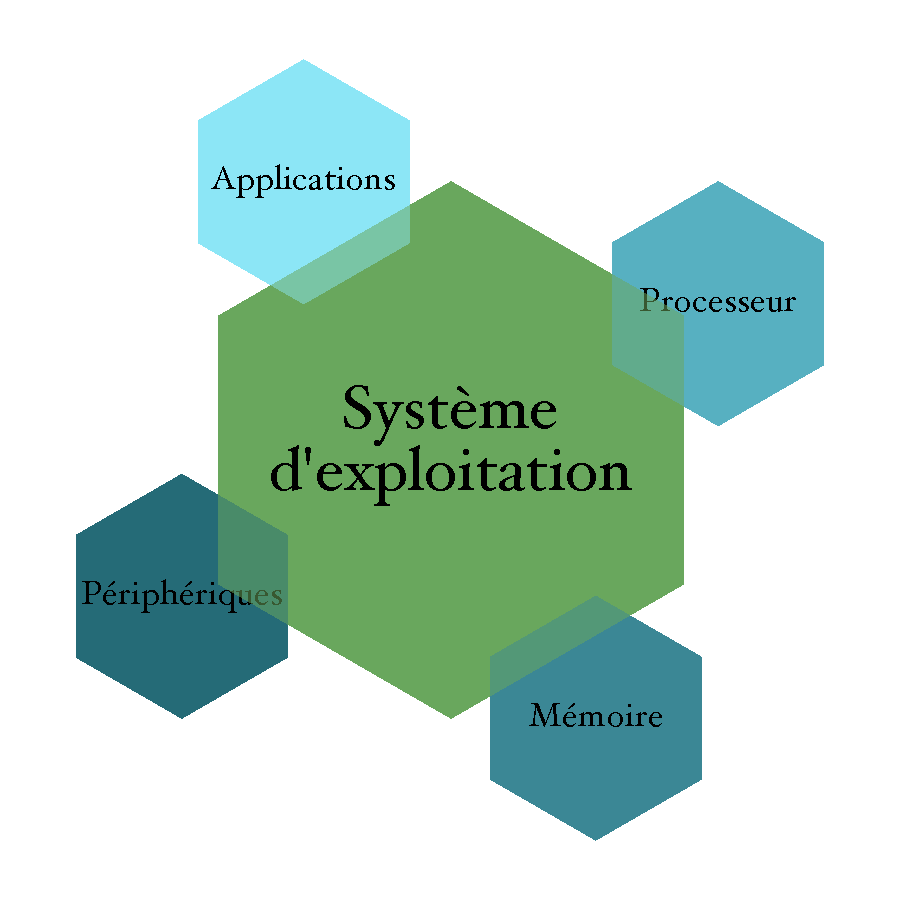
\includegraphics[scale=0.5]
  {textures/images/intro/os.pdf}
	\caption{Relations du système d'exploitation}
\end{figure}

Celui-ci est donc l'intermédiaire entre les logiciels, l'utilisateur et le
matériel (\textit{carte graphique, processeur, mémoire, périphériques, etc.}).
\\ Il gère ainsi la mémoire de l'ordinateur et la répartit entre tous les
programmes. \\ Par conséquent, lorsqu'une application nécessite diverses
informations, il lui suffit de faire appel au système d'exploitation.

\newpage

\subsection{Rôles}
Le système d'exploitation occupe différents rôles : \\

\begin{itemize}
\item \textbf{Gestion du processeur} : l'OS permet de gérer l'allocation du
processeur utile entre les différents programmes. \\

\item \textbf{Gestion de la mémoire vive} : celui-ci permet également
l'allocation de la mémoire utile afin de stocker les données des différentes
applications, ainsi que des différents utilisateurs. \\

\item \textbf{Gestion des entrées/sorties} (\textit{I/O}) : le système
d'exploitation permet de gérer les périphériques tels que des imprimantes,
scanneurs, souris, disques durs, etc. \\

\item \textbf{Gestion de l'exécution des applications} : il gère l'exécution
des applications et leur affecte les ressources nécessaires pour s'exécuter \\

\item \textbf{Gestion des droits} : le système d'exploitation s'assure que
l'application a des restrictions sur l'accès aux fichiers critiques (comme le
dossier \textit{System32} sous Windows) ainsi que les utilisateurs ne possédant
pas les droits adéquats (\textit{session invité}). \\

\item \textbf{Gestion des fichiers} : il gère la lecture ainsi que l'écriture
des fichiers et les droits d'accès aux fichiers par les logiciels et les
utilisateurs. \\

\item \textbf{Gestion des informations} : l'OS avertit l'utilisateur du bon
fonctionnement de l'ordinateur notamment à l'aide d'indicateurs et de logiciels
de diagnostic. \\

\item \textbf{Gestion de l'environnement de bureau} : le système affiche des
fenêtres et des icônes imitant un véritable bureau vu de haut
(\textit{calculatrice, corbeille, documents, ...}). Cette interface permet
d'utiliser facilement un ordinateur. Avant, tout se déroulait en ligne de
commande (\textit{CLI}) à l'aide d'un langage dédié. \\

\item \textbf{Gestion de la sécurité} : c'est à lui de veiller à la sécurité
d'agressions externes (réseau ou périphériques externes) ainsi qu'à la sécurité
de fonctionnement lors de pannes (logicielles ou matérielles). Le système doit
alors sauvegarder automatiquement les fichiers lors de l'arrêt et doit
permettre le redémarrage et la récupération des fichiers.
\end{itemize}

\newpage

\subsection{Différents systèmes d'exploitation}
Il existe un grand nombre de systèmes d’exploitation dédiés à différents
matériels (\textit{ordinateurs, smartphones et tablettes, cartes à puces,
véhicules, robots, équipement réseau, etc.}). \\

Chacun ayant une interface et des logiciels adaptés au matériel pour lequel il
est développé. \\ Les systèmes pour ordinateurs sont adaptés aux grands écrans
et à la navigation clavier-souris, alors que, pour le mobile, ils ont une
interface prévue pour le tactile et des écrans de plus petite taille. \\

Les deux familles de systèmes d'exploitation les plus populaires sont Unix
(principalement \textit{OS X, GNU/Linux, iOS et Android}) et Windows. Cette
dernière détient un quasi-monopole sur les ordinateurs personnels avec près de
90\% de part de marché depuis 15 ans. \\

Il est à noter que, depuis Windows 8, le système de Microsoft est adapté aux
tablettes et autres écrans tactiles (ce n’est pas le cas de Windows pour
smartphones qui est un autre OS nommé Windows Phone et Windows 10 Mobile). \\

Du côté de Apple, le système mobile (iOS anciennement \textit{iPhone OS}) est
un dérivé de Mac OS X. En effet, leur base est commune et leur plus grande
différence réside dans leur interface graphique. \\

Chez GNU/Linux, il existe un grand nombre de systèmes d’exploitation mobiles
(comme \textit{Android, Firefox OS, Tizen ou encore Ubuntu Touch}). \\
Android en est, de loin, le plus connu avec 85\% de part de marché dans le
mobile. \\

Pour les équipements réseau, il existe Cisco IOS qui s'utilise via la ligne
de commande. \\

De manière générale, il existe de nombreux systèmes d'exploitation portant
sur divers domaines. Ceux-ci sont développés pour une technologie bien précise
ce qui explique, entre autres, la multitude de ces OS dans le quotidien. \\
Bien entendu, pour les systèmes d'exploitation mobiles et ceux liés aux
ordinateurs, il y a des incompatibilités en terme de logiciels. Cela signifie
qu'un logiciel qui fonctionne sur un OS peut ne pas s'exécuter correctement sur
un autre.

\newpage

\subsection{Marché des OS}

Voici les parts de marché des systèmes d'exploitation les plus utilisés par
catégorie : \\

\begin{tabular} {p{7cm} p{8cm}}
	\begin{itemize}
  \item[$\bullet$] \textbf{Ordinateurs} (Janvier 2016) :
    \begin{enumerate}
    \item Windows (\textbf{85,18\%})
    \item Mac OS X (\textbf{9,03\%})
    \item GNU/Linux (\textbf{1,47\%})
    \item Chrome OS (\textbf{0,51\%})
    \item Autres (\textbf{3,81\%})
    \end{enumerate}
	\end{itemize}
	& \begin{itemize}
  \item[$\bullet$] \textbf{Smartphones et tablettes} (2014) :
    \begin{enumerate}
    \item Android (\textbf{85\%})
    \item iOS (\textbf{11\%})
    \item Windows Phone (\textbf{2,5\%})
    \item BlackBerry OS (\textbf{1\%})
    \item Autres (\textbf{0,5\%})
    \end{enumerate}
	\end{itemize}
\end{tabular}

En ne gardant que les trois systèmes les plus utilisés de chaque catégorie, on obtient ce classement:

\begin{center}
	\begin{tabular} {p{8cm}} \centering
		\begin{enumerate}
    \item Windows \textit{PC et Mobile} (\textbf{45,15\%})
    \item Android (\textbf{43,77\%})
    \item iOS (\textbf{5,66\%})
    \item Mac OS X (\textbf{4,66\%})
    \item Linux (\textbf{0,76\%})
		\end{enumerate}
	\end{tabular}
\end{center}

\begin{figure}[!h]
  \center
  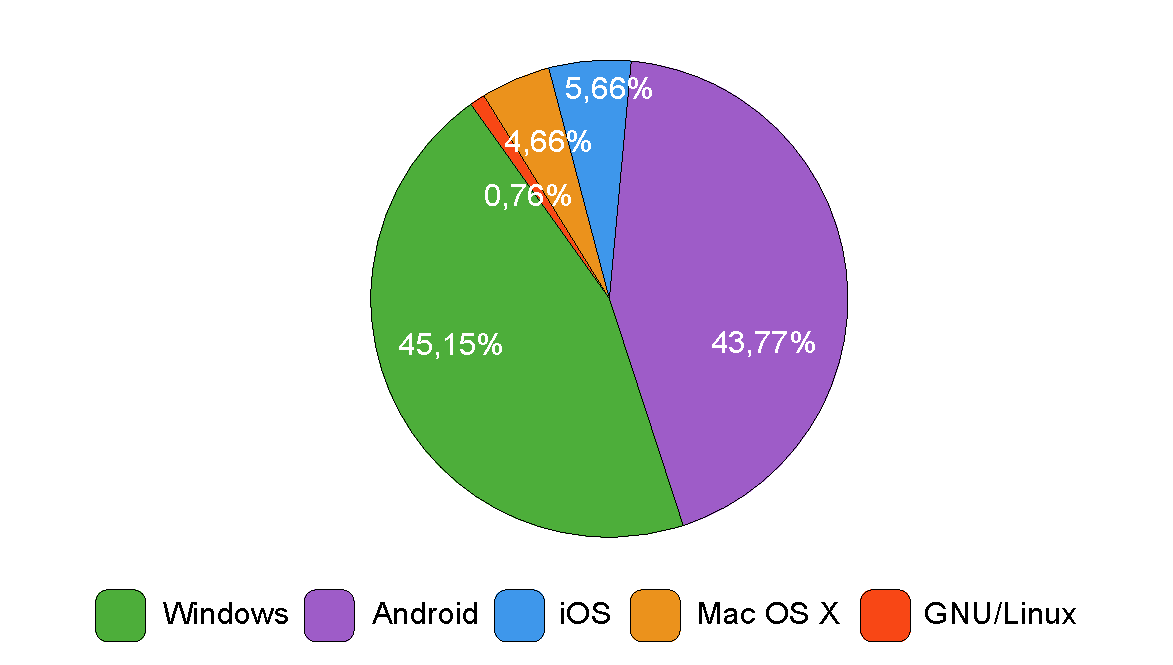
\includegraphics[scale=0.52]
  {textures/images/intro/moreUsedOS.pdf}
  \caption{Statistiques des systèmes d'exploitation plus utilisés}
\end{figure}

\newpage

Par conséquent, les cinq systèmes d'exploitation les plus utilisés sont, dans
l'ordre décroissant : Windows, Android, iOS, Mac OS X et GNU/Linux. \\

Il est à noter qu'aux USA, les parts de marché de Windows ont fortement baissé
en 8 ans : elles sont passées de près de 95\% à 20\%. \\ Microsoft se retrouve
maintenant derrière Google avec Android et Chrome OS (42\%) et Apple avec OS X
et iOS (24\%). \\

Logos de ces différents OS: \\

\begin{figure}[!h]
	\centering
	
\includegraphics[scale=0.1]
	{textures/images/intro/logo/windows.pdf}
	\caption{Logo de Windows}
\end{figure}

\begin{figure}[!h]
	\centering
	
\includegraphics[scale=0.03]
	{textures/images/intro/logo/android.pdf}
	\caption{Bugdroid, la mascotte de Android}
\end{figure}

\begin{figure}[!h]
	\centering
	
\includegraphics[scale=0.03]
	{textures/images/intro/logo/ios.pdf}
	\caption{Logo de iOS}
\end{figure}

\begin{figure}[!h]
	\centering
	
\includegraphics[scale=0.03]
	{textures/images/intro/logo/osx.pdf}
	\caption{Logo de Mac OS X}
\end{figure}

\begin{figure}[!h]
	\centering
	
\includegraphics[scale=0.05]
	{textures/images/intro/logo/tux.pdf}
	\caption{Tux, la mascotte de Linux}
\end{figure}

\newpage
\section{Windows}
\subsection{Historique}
Descendant de MS-DOS (\textit{Microsoft Disk Operating System}) créé en 1981
par Bill Gates, Paul Allen et Steve Ballmer. Ce n'est que le 20 novembre 1985
que la première version de Windows apparut (\textit{Windows 1.0}) offrant la
possibilité d'utiliser une interface graphique sans devoir taper des commandes
MS-DOS. \\

20 jours plus tard, Windows 2.0 voit le jour offrant la possibilité de faire se
chevaucher des fenêtres, de contrôler la disposition de l'écran ainsi que de
faire l'usage de raccourcis clavier. En 1988, les ordinateurs commencent à
faire partie du quotidien de divers employés de bureau. \\

Windows 3.0 fut annoncé le 22 mai 1990 et la version 3.1 sera disponible en
1992. Suite à cela, Windows dispose désormais de meilleures performances d'un
point de vue graphismes puisqu'il peut supporter 16 couleurs et possède une
amélioration concernant les icônes. \\

Remarque : Windows NT, sorti le 27 juillet 1993, sera intéressant d'un point de
vue commercial puisque celui-ci est un système d'exploitation 32 bits. \\

Dans la suite de l'évolution, Windows 95 sort le 24 août 1995 offrant les
fonctionnalités de base que nous connaissons aujourd'hui tel que le bouton
Démarrer, l'heure des fax/modems, du courrier électronique, de l'univers en
ligne et des jeux multimédias et logiciels éducatifs, ... \\

À ce moment, 80 \% des PC du monde entier utilisent Windows et MS-DOS. \\

Le 25 juin 1998, Windows 98 est rendu disponible et devient la première
version de Windows spécialement conçue pour les utilisateurs. Les PC sont dès à
présent disponibles tout autour de nous, que ce soit dans les bureaux, à la
maison ou dans des cybercafés. Cette version sera la dernière version basée sur
MS-DOS. \\

Toujours dans l'utilisation domestique, Windows Me proposera des \\
perfectionnements pour la musique, la vidéo et le réseau domestique, ... \\

Dès lors, Microsoft annonce que tous les prochains systèmes d'exploitation
seront basés sur le noyau de Windows NT et de Windows 2000. \\

Windows 2000 Professionnel simplifie entre autres l'installation matérielle en
considérant la prise en charge de matériels Plug-and-Play, comprenant des
produits sans fil et réseau, des périphériques USB, des périphériques IEEE-1394
et des périphériques infrarouges. \\

L'un des produits les plus vendus au cours des prochaines années sera Windows
XP disponible à partir du 25 octobre 2001 et qui sera proposé en plusieurs
versions (64 bits, Media Center, Tablet PC). Effectivement, celui-ci sera
fourni dans 25 langues et offrant une nouvelle ergonomie ciblée sur
l'utilisation et le centre unifié de services d'aide et d'assistance. \\

En 2006, Windows Vista est annoncé visant à renforcer la sécurité à l'aide d'un
contrôle de compte d'utilisateur, en apportant un lecteur de chiffrement
BitLocker, ... \\

Néanmoins, cette version de Windows fut beaucoup critiquée suite aux nombreux
logiciels provenant de Windows XP incompatibles avec cette version. \\

En 2009, Microsoft introduit l'interface tactile à l'aide de Windows 7 vu qu'il
est devenu courant de se connecter dans des zones d'accès sans fil. \\

Suivant cette direction, Windows 8 - conçu en 2012 - propose une toute nouvelle
interface compatible à la fois avec un clavier et une souris ainsi qu'avec la
technologie tactile. \\

Puis, après la version Windows 8.1, Windows 10 est enfin arrivé et est, d'après
Microsoft, le meilleur Windows jamais créé. Cette version dispose d'une
assistante personnelle intelligente (\textit{Cortana}). \\

\begin{figure}[!htb] \minipage{0.45\textwidth}
  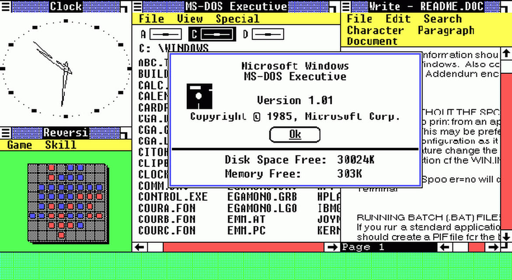
\includegraphics[width=\linewidth]{textures/images/windows/historic/Win1.png}
  \caption{Windows 1.01}\label{fig:Windows 1.01}
	\endminipage\hfill \minipage{0.45\textwidth}
  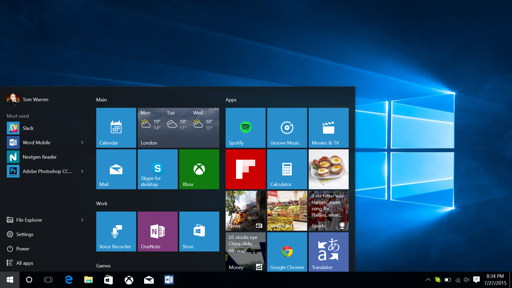
\includegraphics[width=\linewidth]{textures/images/windows/historic/Win10.png}
  \caption{Windows 10}\label{fig:Windows 10}
	\endminipage
\end{figure}

\clearpage

\subsection{Utilisation}
Windows étant le premier système d'exploitation pour les PC en terme de part de
marché, il est aisé de savoir le pourquoi du comment de cette position. \\

Premièrement, il faut savoir que Windows est le système d'exploitation installé
par défaut sur tous les ordinateurs. De ce fait, lors de l'achat de
l'ordinateur, Windows est fourni avec celui-ci. \\

Remarque : il est possible d'acheter un ordinateur directement avec GNU/Linux
sur des sites commerciaux en technologie tels que \textit{LDLC} et
\textit{system76}, ce qui permet de réduire le prix initial de l'ordinateur. \\

De plus, la plupart des développeurs s'occupent en priorité de la compatibilité
sur Windows permettant de rendre leurs logiciels accessibles pour un public
beaucoup plus vaste. \\

Windows a également l'avantage de regrouper diverses catégories de personne. On
y retrouve des adolescents dont leur demande première se trouve dans
l'utilisation de jeux vidéo, des adultes voulant profiter des fonctionnalités
standards qu'offre un système d'exploitation, des personnes âgées, ... \\

Autrement dit, Windows est un système d'exploitation universel regroupant une
large communauté de personnes ce qui offre l'avantage de trouver une réponse
très facilement face à un problème ou une question spécifique sur l'OS. \\

Il est également possible d'utiliser cet OS sur son téléphone.
Effectivement, des smartphones sont équipés de Windows Phone. Même si celui-ci
est moins répandu qu'Android et iOS, il a l'avantage d'être très rapide sur de
petites configurations et d'offrir des téléphones à prix raisonnable. La
principale raison à cela est que de nombreuses applications ne fonctionnent que
pour Android ou iOS. \\

Néanmoins, certains spécialistes en la matière considèrent que Windows Phone
n'est pas rentable pour Microsoft et qu'il ne sera plus mis à jour dans le
futur. De ce fait, les utilisateurs de Windows Phone devront opter pour Android
ou iOS si ça devait être le cas.

\clearpage

\subsection{Mobile}

Tout comme Apple, Nokia et Samsung, Microsoft possède une longue histoire dans
le mobile. Entre les PDA, les tablettes et les téléphones, ces firmes ont
développé des systèmes d'exploitation mobiles spécialement conçus pour ces
appareils. \\

La première version de ce système est nommée \textit{Pocket PC 200} et est basée
sur une version de Windows spécialement prévue pour des appareils possédant
peu de ressources - Windows CE. \\

Au fil des ans, le nom devient Windows Mobile 2003 puis Windows Mobile 5. Sur
cette version, on peut retrouver une adaptation de Microsoft Office. \\

Avec la sortie de l'iPhone en 2007 suivi très rapidement par Samsung (avec Android),
Windows Mobile est à la traîne. C'est pourquoi Microsoft présente Windows Phone 7
au public en 2011. Pendant ce temps, Windows Mobile 6 a connu de grands changements
afin de rester dans la course…

  \begin{figure}[!h]
    \center
    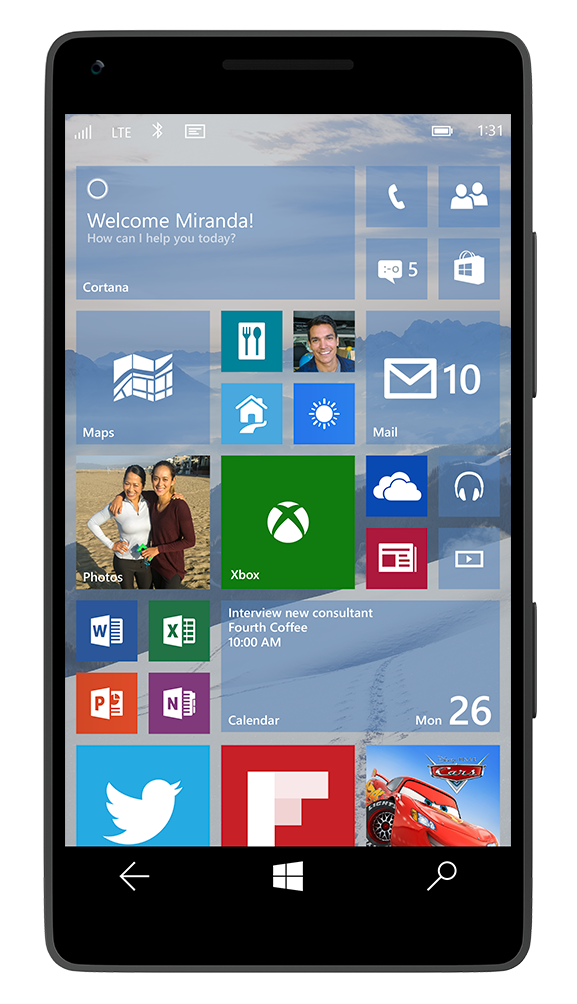
\includegraphics[scale=0.5]
    {textures/images/windows/Windows10Mobile.png}
    \caption{Windows 10 Mobile}
  \end{figure}

La dernière version en date est Windows Mobile 10 qui est très proche de la
version bureau, la politique de Microsoft étant d'avoir un seul et unique
système d'exploitation pour tous les appareils.

\newpage

\subsection{Fonctionnalités}
Le système d'exploitation de la firme de Redmond possède plusieurs fonctionnalités bien à lui. \\

Depuis Windows 10, les applications disponibles dans le Windows Store sont
universelles. Elles peuvent donc tourner sur n'importe quel ordinateur ou
smartphone possédant Windows 10, ainsi que sur les Xbox One et les \textit{HoloLens} ! \\
La suite Microsoft Office est d'ores et déjà universelle. \\

Une autre nouveauté se nomme \textit{Continuum} et consiste à « transformer » sa tablette tantôt en
ordinateur portable, tantôt en tablette. \\
L'utilisateur peut utiliser sa tablette en tant que PC, avec son clavier et une souris,
avec la version PC de Windows 10; puis l'utiliser en \textit{mode tablette}:
le menu Démarrer prend tout l'écran comme dans Windows 8. \\
Pour les Windows Phones, il existe quelque chose de similaire: si l'on branche son
Windows Phone - \textit{muni de Windows 10 Mobile} - à un clavier, une souris et sa station d'accueil
elle-même branchée à un écran, l'écran susmentionné affiche une interface de bureau. Le système
est encore celui de Windows Mobile mais il affiche un menu Démarrer et un \textit{faux} bureau.
Bien entendu, seules les applications universelles peuvent être utilisées dans ce mode. \\

Pour les joueurs possédant une Xbox One, il est possible d’y jouer depuis son ordinateur sous Windows 10. \\

Côté sécurité, depuis Windows 8, il est possible de se connecter à l’aide d’un code à 4 chiffres
comme sur mobiles ou un code gestuel sur une image.
Avec l’arrivée de Windows 10, \textit{Windows Hello} fait son apparition.
La connexion peut s'effectuer à l’aide d’un capteur biométrique, le critère est
désormais le visage (\textit{à l’aide d’une caméra RealSense 3D}), une empreinte digitale ou l’iris.

\begin{figure}[!htb] \minipage{0.45\textwidth}
  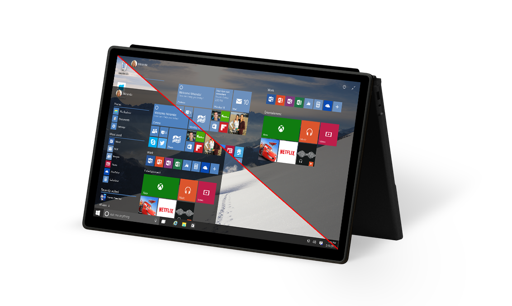
\includegraphics[width=\linewidth]
  {textures/images/windows/features/Continuum_tablet.png}
  \caption{Continuum tablette}\label{fig: Continuum}
	\endminipage\hfill \minipage{0.45\textwidth}
  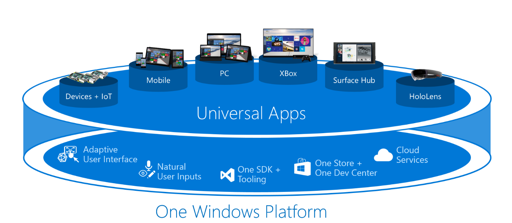
\includegraphics[width=\linewidth]{textures/images/windows/features/Universal_App.png}
  \caption{App universelle}\label{fig:App universelle}
	\endminipage
\end{figure}

\clearpage

\newpage
\section{Unix}
\subsection{Historique}
Créé en 1969 par Ken Thompson et Dennis Ritchie suite à l'idéologie qu'un
système d'exploitation performant pour un usage interactif n'avait nul besoin
d'être coûteux, que ce soit en termes d'ordinateur d'accueil ou de développement
humain. Néanmoins, ce n'est qu'en octobre 1973 qu'UNIX prendra sa place au sein
du monde informatique, les codes sources furent disponibles et modifiables par
la communauté qui apporta à UNIX de meilleurs outils. De nos jours, UNIX fait
partie des systèmes d'exploitation les plus répandus bien qu'il ait été conçu
et développé il y a quelques dizaines d'années. \\

Les principales raisons faisant qu'UNIX soit encore utilisé aujourd'hui sont
notamment dues à sa robustesse et à quelques fonctionnalités bien élaborées dès
sa conception. De plus, celui-ci possède l'avantage de n'être lié à aucune
architecture ni aucun constructeur particulier. Il en existe de nombreuses versions,
y compris les \textit{UNIX-like} qui s'autoproclament être un système
d'exploitation parfaitement compatible avec UNIX en n'ayant jamais obtenu la
spécification UNIX. Parmi eux, on y trouve la plupart de systèmes gratuits
et/ou open source dont les plus connus sont GNU/Linux et FreeBSD. \\

Ces versions ont l'avantage de pouvoir exploiter la quasi-totalité du matériel
informatique disponible sur le marché que ce soit sur des serveurs volumineux,
de gros calculateurs ou des ordinateurs domestiques. De même, divers boîtiers
réseau (\textit{routeurs, switches, ...}) fonctionnent sous UNIX et certains
ordinateurs de poche (\textit{PDA}) et smartphones sont équipés d'UNIX. \\

Cependant, avant les années 1990, UNIX n'a été disponible que dans le monde
scientifique avec une interface utilisateur austère. Suite à l'apport du
protocole graphique X-Window développé par le MIT, tout utilisateur peut
utiliser une station UNIX à l'aide d'une souris et d'un écran graphique, même
s'il est recommandé d'apprendre le fonctionnement interne ainsi que des
commandes spécifiques afin d'exploiter au maximum les possibilités d'UNIX,
notamment pour les administrateurs système qui doivent souvent développer des
scripts afin d'automatiser certaines tâches. \\

En 1991, Linus Torvalds - étudiant en informatique à l'Université d'Helsinki -
conçoit le noyau Linux suite à une déception du système d'exploitation MS-DOS
et à cause d'un manque de bonne émulation de terminal proposé par MINIX, un
clone open source d'UNIX développé par Andrew Tanenbaum.

\newpage

\subsection{Composition}
Le système d'exploitation UNIX comporte un ensemble d'outils mis à disposition
de l'utilisateur, et son rôle principal est la répartition automatique des
ressources de manière équitable entre les différentes tâches et utilisateurs. \\
Globalement, UNIX est composé des éléments suivants : \\

\begin{itemize}
\item Un noyau dont le rôle est d'assurer la gestion de la mémoire, les
échanges d'entrées/sorties de bas niveau ainsi que de la répartition des
tâches. \\

\item Un ensemble d'utilitaires de base : \\

  \begin{itemize}
  \item[$\bullet$] Divers interpréteurs de commande qui permettent d'exécuter
des commandes utiles à la manipulation de fichiers, de gestion de processus
(\textit{activité du système}), de communications (\textit{tubes, sockets
TCP/IP intégrés}), ... De plus, ces interpréteurs permettent de démarrer des
activités séparées ou communicantes. \\

  \item[$\bullet$] Des éditeurs de textes (\textit{nano, vim}). \\

  \item[$\bullet$] Des compilateurs ainsi que des éditeurs de liens. Néanmoins,
depuis la fermeture des codes sources, le compilateur C n'est plus inclus dans
aucune distribution UNIX. \\

  \item[$\bullet$] Des outils généraux de développement. \\

  \item[$\bullet$] Des utilitaires résidents (\textit{démons}) chargés de rendre
un certain nombre de services de manière transparente.
  \end{itemize}

  \begin{figure}[!h]
    \centering
    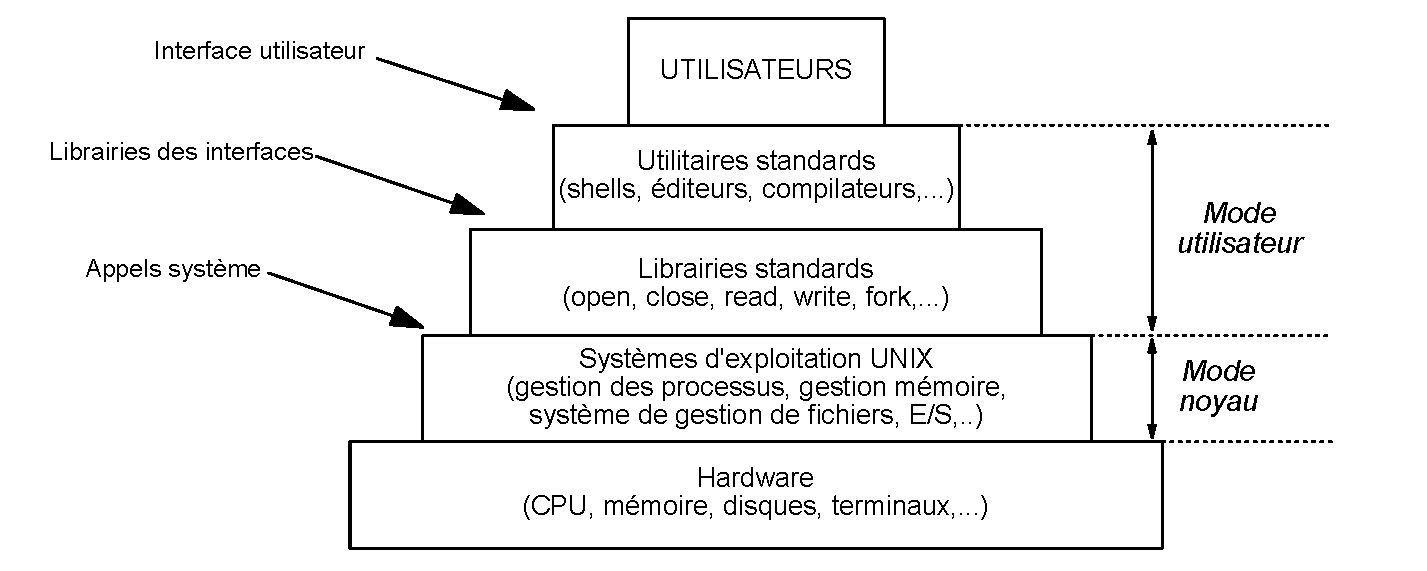
\includegraphics[scale=0.5]
    {textures/images/unix/composition.pdf}
    \caption{Composition d'UNIX}
  \end{figure}
\end{itemize}

\clearpage

\subsection{Distributions}
Elles sont composées d'un ensemble de logiciels définis en fonction de la
distribution choisie et d'un système d'exploitation comportant un noyau. Linux
en possède un très grand nombre en fonction des besoins de l'utilisateur. \\

Exemples de distributions : \\

\begin{itemize}
\item Ubuntu : distribution fournissant un système convivial et ergonomique
pour le grand public. Celui-ci ne nécessite pas de réelles connaissances
approfondies. Elle est recommandée pour un utilisateur désirant apprivoiser les
fonctionnalités de base qu'offre GNU/Linux.

\begin{figure}[!h]
  \center
  
\includegraphics[scale=0.3]
  {textures/images/unix/logos/ubuntu.pdf}
  \caption{Ubuntu}
\end{figure}

\item Red Hat : distribution orientée serveurs et destinée à un public
professionnel. Elle est souvent utilisée par les entreprises.

\begin{figure}[!h]
  \center
  
\includegraphics[scale=0.5]
  {textures/images/unix/logos/redhat.pdf}
  \caption{Red Hat}
\end{figure}

\item Debian : probablement la distribution la plus populaire dont les maîtres
mots sont la stabilité et l'efficacité. Elle concerne un public limité
ayant des notions de base sur GNU/Linux. Seul l'indispensable est
installé par défaut, offrant l'opportunité à l'utilisateur une indépendance par
rapport à sa configuration.

\begin{figure}[!h]
  \center
  
\includegraphics[scale=0.7]
  {textures/images/unix/logos/debian.pdf}
  \caption{Debian}
\end{figure}

\item Fedora : distribution communautaire de Red Hat dont la caractéristique
  première est de suivre les nouveautés technologies. Similaire à Ubuntu, elle
  concerne un grand public et ne nécessite pas de connaissances sur
  GNU/Linux.

\begin{figure}[!h]
  \center
  
\includegraphics[scale=0.5]
  {textures/images/unix/logos/fedora.pdf}
  \caption{Fedora}
\end{figure}

\item Arch Linux : comme Debian, cette distribution - fournissant peu
d'utilitaires d'aide à la configuration - est destinée aux utilisateurs avancés.
Celle-ci sera privilégiée si l'utilisateur veut un système d'exploitation
rapide, léger et flexible. \\

\begin{figure}[!h]
  \center
  
\includegraphics[scale=1.4]
  {textures/images/unix/logos/archlinux.pdf}
  \caption{Arch Linux}
\end{figure}

\item Slackware : c'est la plus vieille des distributions encore utilisées dont l'idéologie est d'être rapide et sans fioritures. Souvent utilisée sur des serveurs, celle-ci n'est maintenue que par très peu de monde dans l'entourage de son
fondateur. \\

\begin{figure}[!h]
  \center
  
\includegraphics[scale=0.5]
  {textures/images/unix/logos/slackware.pdf}
  \caption{Slackware}
\end{figure}

\item (...) \\
\end{itemize}

\newpage

\subsection{Environnements de bureau}
À ne pas confondre avec le système d'exploitation qui s'occupe de gérer les
ressources de l'ordinateur, l'environnement de bureau constitue les
caractéristiques graphiques du système d'exploitation. C'est lui qui permet à
l'utilisateur d'interagir avec son ordinateur. \\

Celui-ci est constitué de divers éléments : \\

\begin{itemize}
\item Bureau : affichage d'un arrière-plan ainsi que d'un ensemble d'icônes. \\

\item Gestionnaire de fenêtres : délimitations des fenêtres par des cadres. \\

\item Barres de menu et des panneaux associés : offre l'accès aux logiciels, à
l'heure, de lister les fenêtres en cours, ... \\

\item Gestionnaire de session : s'occupe des sessions de l'ordinateur. \\

\item Outils graphiques: permettent de contrôler l'ordinateur. \\
\end{itemize}

Divers environnements de bureau : \\

\begin{figure}[!htb]
  \minipage{0.4\textwidth}
  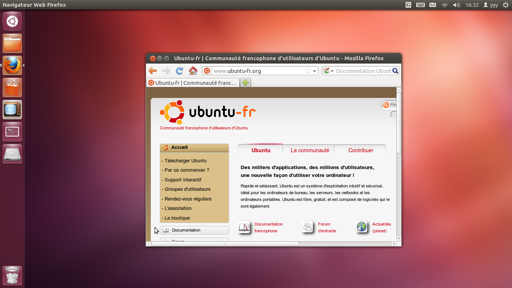
\includegraphics[width=\linewidth]{textures/images/unix/desktop_environment/unity.png}
  \caption{Unity}\label{fig:unity}
  \endminipage\hfill
  \minipage{0.4\textwidth}
  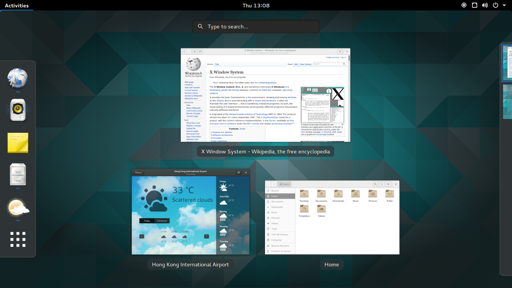
\includegraphics[width=\linewidth]{textures/images/unix/desktop_environment/gnome-shell.png}
  \caption{Gnome Shell}\label{fig:gnome shell}
  \endminipage
\end{figure}

\begin{figure}[!htb]
  \minipage{0.4\textwidth}
  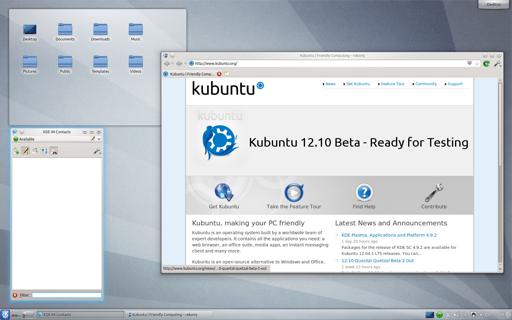
\includegraphics[width=\linewidth]{textures/images/unix/desktop_environment/kde.png}
  \caption{KDE}\label{fig:kde}
  \endminipage\hfill
  \minipage{0.4\textwidth}
  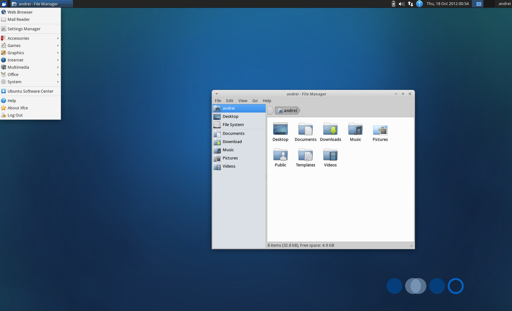
\includegraphics[width=\linewidth]{textures/images/unix/desktop_environment/xfce.png}
  \caption{XFCE}\label{fig:xfce}
  \endminipage
\end{figure}

\newpage

\subsection{Mobilité}
Chez GNU/Linux, il existe un grand nombre de systèmes d’exploitation mobiles et
Android en est le plus connu. Pour tout dire, c'est même le plus utilisé des
systèmes d'exploitation pour smartphones et tablettes avec ses 85 \% de parts de
marché mobile dans le monde. \\

Basé sur un noyau Linux et développé par \textit{Android, Inc.}, il est conçu
pour les smartphones et les tablettes. Trois ans après le rachat de l'entreprise
par Google, le premier smartphone Android - le \textit{T-Mobile G1} - sort aux
États-Unis. Cette première version met en place la \textit{marque de fabrique}
de la plateforme comme les widgets, le Android Market (maintenant nommé
\textit{Play Store}) et l'intégration avancée de Gmail. \\

Le système étant distribué à tout constructeur, Android se trouve être le pendant
de Windows sur mobile: la majorité des mobiles tourne sous une version de Android.
Ce n'est donc pas un hasard si le pourcentage d'utilisation de Windows sur
ordinateurs et quasiment identique à celui de Android. \\

Avec le temps, Android a gagné en fonctionnalités et peut tourner sur encore plus
de dispositifs, comme des télévisions (\textit{Android TV}), des voitures
(\textit{Android Auto}), des smartwatches (\textit{Android Wear}) ainsi que des
ordinateurs (\textit{Android-x86}). \\

Nous en sommes désormais à la sixième version qui se nomme \textit{Marshmallow}.
L'une des particularités est que chaque version possède un nom de sucrerie et
qu'elles se suivent dans l'ordre alphabétique. En voici quelques: \textit{Cupcake},
\textit{Donut}, \textit{Eclair} et \textit{Jelly Bean}, \textit{KitKat}, etc.

  \begin{figure}[!h]
    \centering
    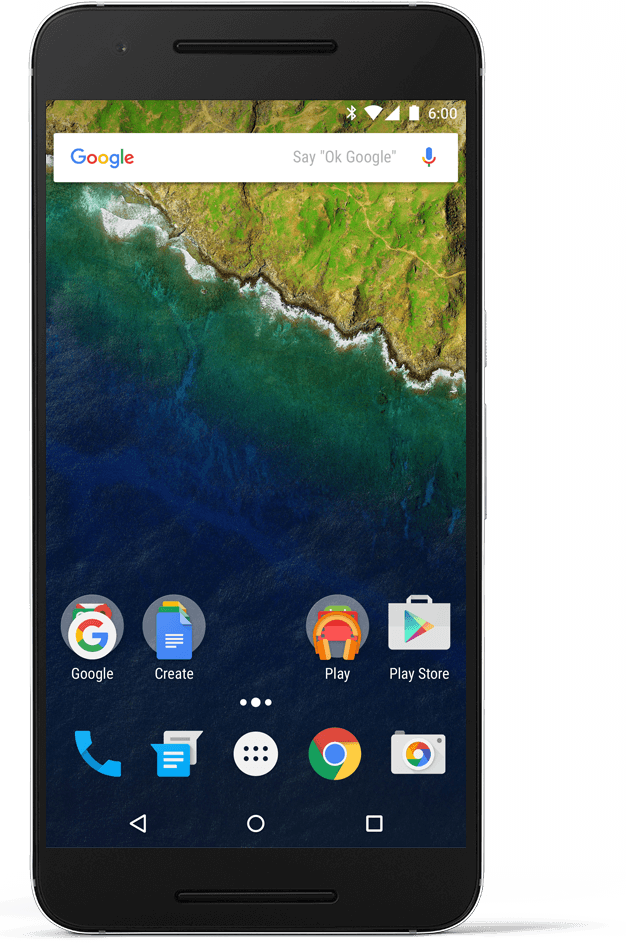
\includegraphics[scale=0.16]
    {textures/images/unix/mobiles/nexus}
    \caption{Nexus 6P sous Android 6.0 Marshmallow}
  \end{figure}

\clearpage
Contrairement aux autres acteurs du marché, GNU/Linux se finance \\
principalement à l'aide de donations, ce qui peut poser divers problèmes pour le
financement de leur développement.  \\

Malgré tout ça, GNU/Linux commence à s'intéresser aux smartphones ainsi qu'aux
tablettes. En effet, Ubuntu Touch est un système d'exploitation développé
pour ces dispositifs. \\

Canonical a d'ailleurs annoncé depuis peu le smartphone « Meizu PRO 5 Ubuntu
Edition » qui est disponible depuis mars 2016.

  \begin{figure}[!h]
    \center
    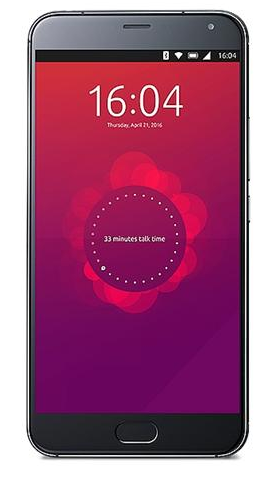
\includegraphics[scale=0.4]
    {textures/images/unix/mobiles/ubuntuTouch}
    \caption{Meizu Pro 5 Ubuntu Edition}
  \end{figure}

Ubuntu Touch à opté pour le glissement de doigt sur l’écran. Un simple
glissement en plein centre de l’écran vers la droite ou la gauche offre la
possibilité de switcher entre les applications principales (\textit{Scopes}).
Et un glissement partant de la bordure de la dalle tactile, ouvre un menu
multitâche similaire à Android. \\

Vu que le système d'exploitation est récent, il est difficile de se prononcer
sur le succès de celui-ci. Cependant, comme Android occupe la majorité du marché
et que celui-ci est composé du noyau Linux, cela sous-entend que cette
technologie pourrait plaire aux utilisateurs d'Android qui désirent d'une
nouvelle interface graphique.

\newpage
\section{Mac OS}
\subsection{Histoire}
C'est en 1976 que le Apple Computer 1, rétroactivement appelé Apple I, est mis
en vente par la \textit{Apple Computer Company} - maintenant appelée
\textit{Apple Inc.} et créée le 1er avril 1976. \\
C'est alors l'un des tout premiers micro-ordinateurs individuels. \\

Alors que Steve Jobs en fait la publicité, il est construit à la main par Steve
Wozniak qui en créa le langage assembleur en BASIC (\textit{en ne passant que
par de l'hexadécimal}) afin de pouvoir programmer des jeux et y jouer. \\
En effet, l'Apple I était principalement fait pour jouer. \\

L'Apple II sort un an plus tard, le système est le même et donne la possibilité
à tous de créer des programmes utilisant les toutes dernières nouveautés: la
couleur et le son. Cependant, il y avait un gros inconvénient: les utilisateurs
devaient stocker leurs données sur des cassettes, cette méthode étant, on s'en
doute, très lente, incommode et peu fiable.

\begin{figure}[!htb] \minipage{0.45\textwidth}
  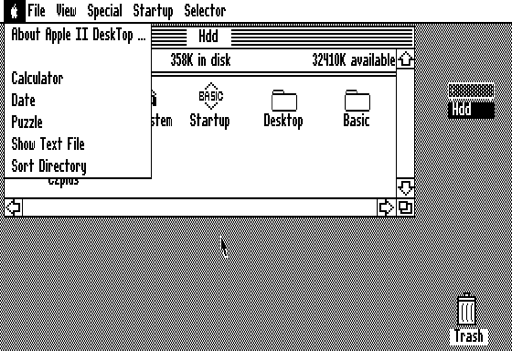
\includegraphics[width=\linewidth]{textures/images/mac/historic/apple2.png}
  \caption{Apple II Desktop}\label{fig:Apple II Desktop}
	\endminipage\hfill \minipage{0.45\textwidth}
  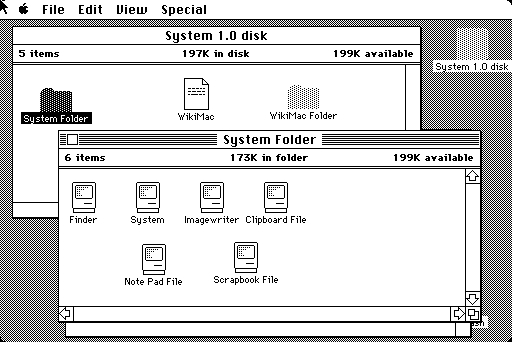
\includegraphics[width=\linewidth]{textures/images/mac/historic/system1.png}
  \caption{System 1}\label{fig:System 1}
	\endminipage
\end{figure}

Pour régler ce problème, le DOS 3.1 (\textit{Disk Operating System}) est rendu
disponible en 1978 et sera mis à jour jusqu'en 1980 avec la version 3.3. \\
Le système d'exploitation permet d’utiliser des disques durs et des disquettes
comme périphériques de stockage. \\

Comme le dit si bien l'adage : "\textit{Jamais deux sans trois.}". La même
année, sort l'Apple III accompagné du SOS (\textit{Sophisticated Operating
System}). \\ C'est le premier OS pour micro-ordinateur à utiliser le
concept de drivers qui aident l’ordinateur à communiquer avec les périphériques
(\textit{disques durs, clavier, écran}), ce qui lui offrit une flexibilité à
utiliser de nouvelles technologies.

\newpage

Une mise à jour du système d'exploitation des Apple II arrive en 1983, ProDOS
(\textit{Professional Disk Operating System}) utilise la même structure de
fichiers que SOS ce qui permet d’utiliser un même disque sur un Apple II et sur
un Apple III, ainsi que de partager des fichiers entre ces ordinateurs. ProDOS
ajoute aussi la compatibilité avec un plus grand nombre de disquettes et
disques durs et augmente le volume maximum de 400 kb à 32 Mb. \\

La même année sort le Lisa avec le Lisa OS qui prend en charge le multitâche et
la protection de mémoire (\textit{droit d’accès à la mémoire non allouée}). \\
De ce fait, le système de fichiers s’améliore encore et devient plus pratique
pour les disques durs à « grande capacité ». \\

Après le Lisa, vient le Macintosh avec le System 1. Les premiers Macintosh ont
utilisé des versions successives du \textit{System} numérotées de 1 à 7. C’est
à partir de la version 7.6 qu’il prend le nom de \textit{Mac OS}. La version
actuelle étant la dixième version majeure ainsi que la version UNIX du système,
son nom est devenu Mac OS X (\textit{Mac OS Ten}). \\

En effet, c'est depuis 1999 et le premier iMac que le système d'exploitation
des ordinateurs Apple est Mac OS X. Il a évolué de la version 10.0
(\textit{Cheetah}) à la version actuelle 10.11 (\textit{El Capitan}). \\

Mac OS X est la fusion entre Mac OS et NeXTSTEP (le système d’exploitation
orienté objet de \textit{NeXT}, l’entreprise fondée par Steve Jobs après son
départ en 1985). NeXTSTEP était un UNIX-like vu que basé sur un noyau Mach et
sur l’implémentation BSD d’UNIX.  \\

Depuis la version 10.5 (en 2007), le système d’exploitation possède la
certification UNIX.

\begin{figure}[!htb]
	\minipage{0.45\textwidth}
  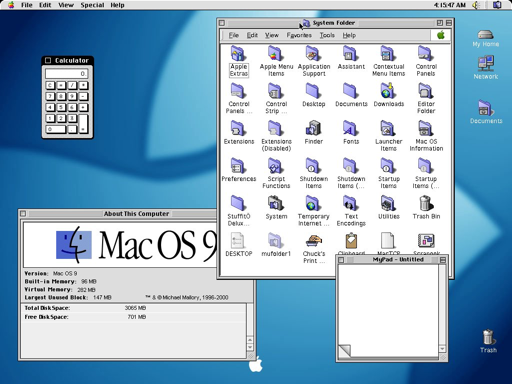
\includegraphics[width=\linewidth]{textures/images/mac/historic/macos9.png}
  \caption{Mac OS 9}\label{fig:OS 9}
	\endminipage\hfill
	\minipage{0.5\textwidth}
  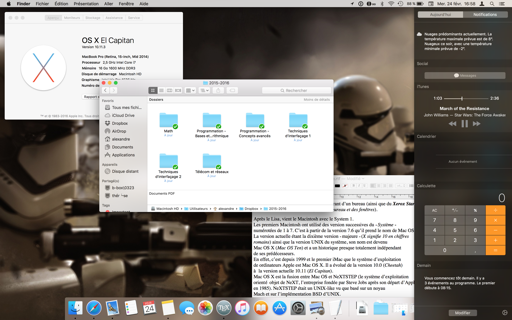
\includegraphics[width=\linewidth]{textures/images/mac/historic/macosx11.png}
  \caption{Mac OS X 10.11}\label{fig:OS X}
	\endminipage
\end{figure}

\subsection{Dérivés}

Même si elle n’est pas très connue, Apple propose une version pour serveur de
son système d’exploitation pour ordinateurs. \textit{Mac OS X Server} est rendu
disponible en tant que mise à jour téléchargeable et prend la forme d’une
simple application. Elle permet de gérer facilement des ordinateurs,
calendriers, fichiers, sauvegardes, etc. \\

Apple possède encore trois autres systèmes d’exploitation - iOS, watchOS et
tvOS basés sur Mac OS X. \\ Comme leur nom l’indique, watchOS est le système de
l’Apple Watch et tvOS est celui de l’Apple TV. iOS est celui des
\textit{iDevices} c’est-à-dire les iPhone, iPad et iPod Touch, son nom vient de
iPhoneOS devenu iOS en 2010, lors de la sortie du premier iPad. \\

Leur base étant la même, certaines applications n’ont pas besoin d’être
entièrement réécrites pour être portées sur une autre plateforme
(\textit{celles d'Apple tout du moins}). Par exemple, l’app Photos sur Mac OS X
n’a pas nécessité beaucoup de changements pour être portée sur iOS. \\

De plus, certaines fonctionnalités comme les fenêtres peuvent être affichées
sur des iPad en activant certains paramètres internes cachés d’iOS. \\

Ces deux OS : Mac OS X et iOS partageant de plus en plus de fonctions, ce
seront bientôt deux systèmes ayant les mêmes fonctionnalités adaptées à leur OS
(\textit{p. ex. écran tactile pour les iDevices}). En effet, pour l’instant il
n’est pas question de fusion, mais plutôt de convergence entre ces deux OS.

  \begin{figure}[!h]
    \center
    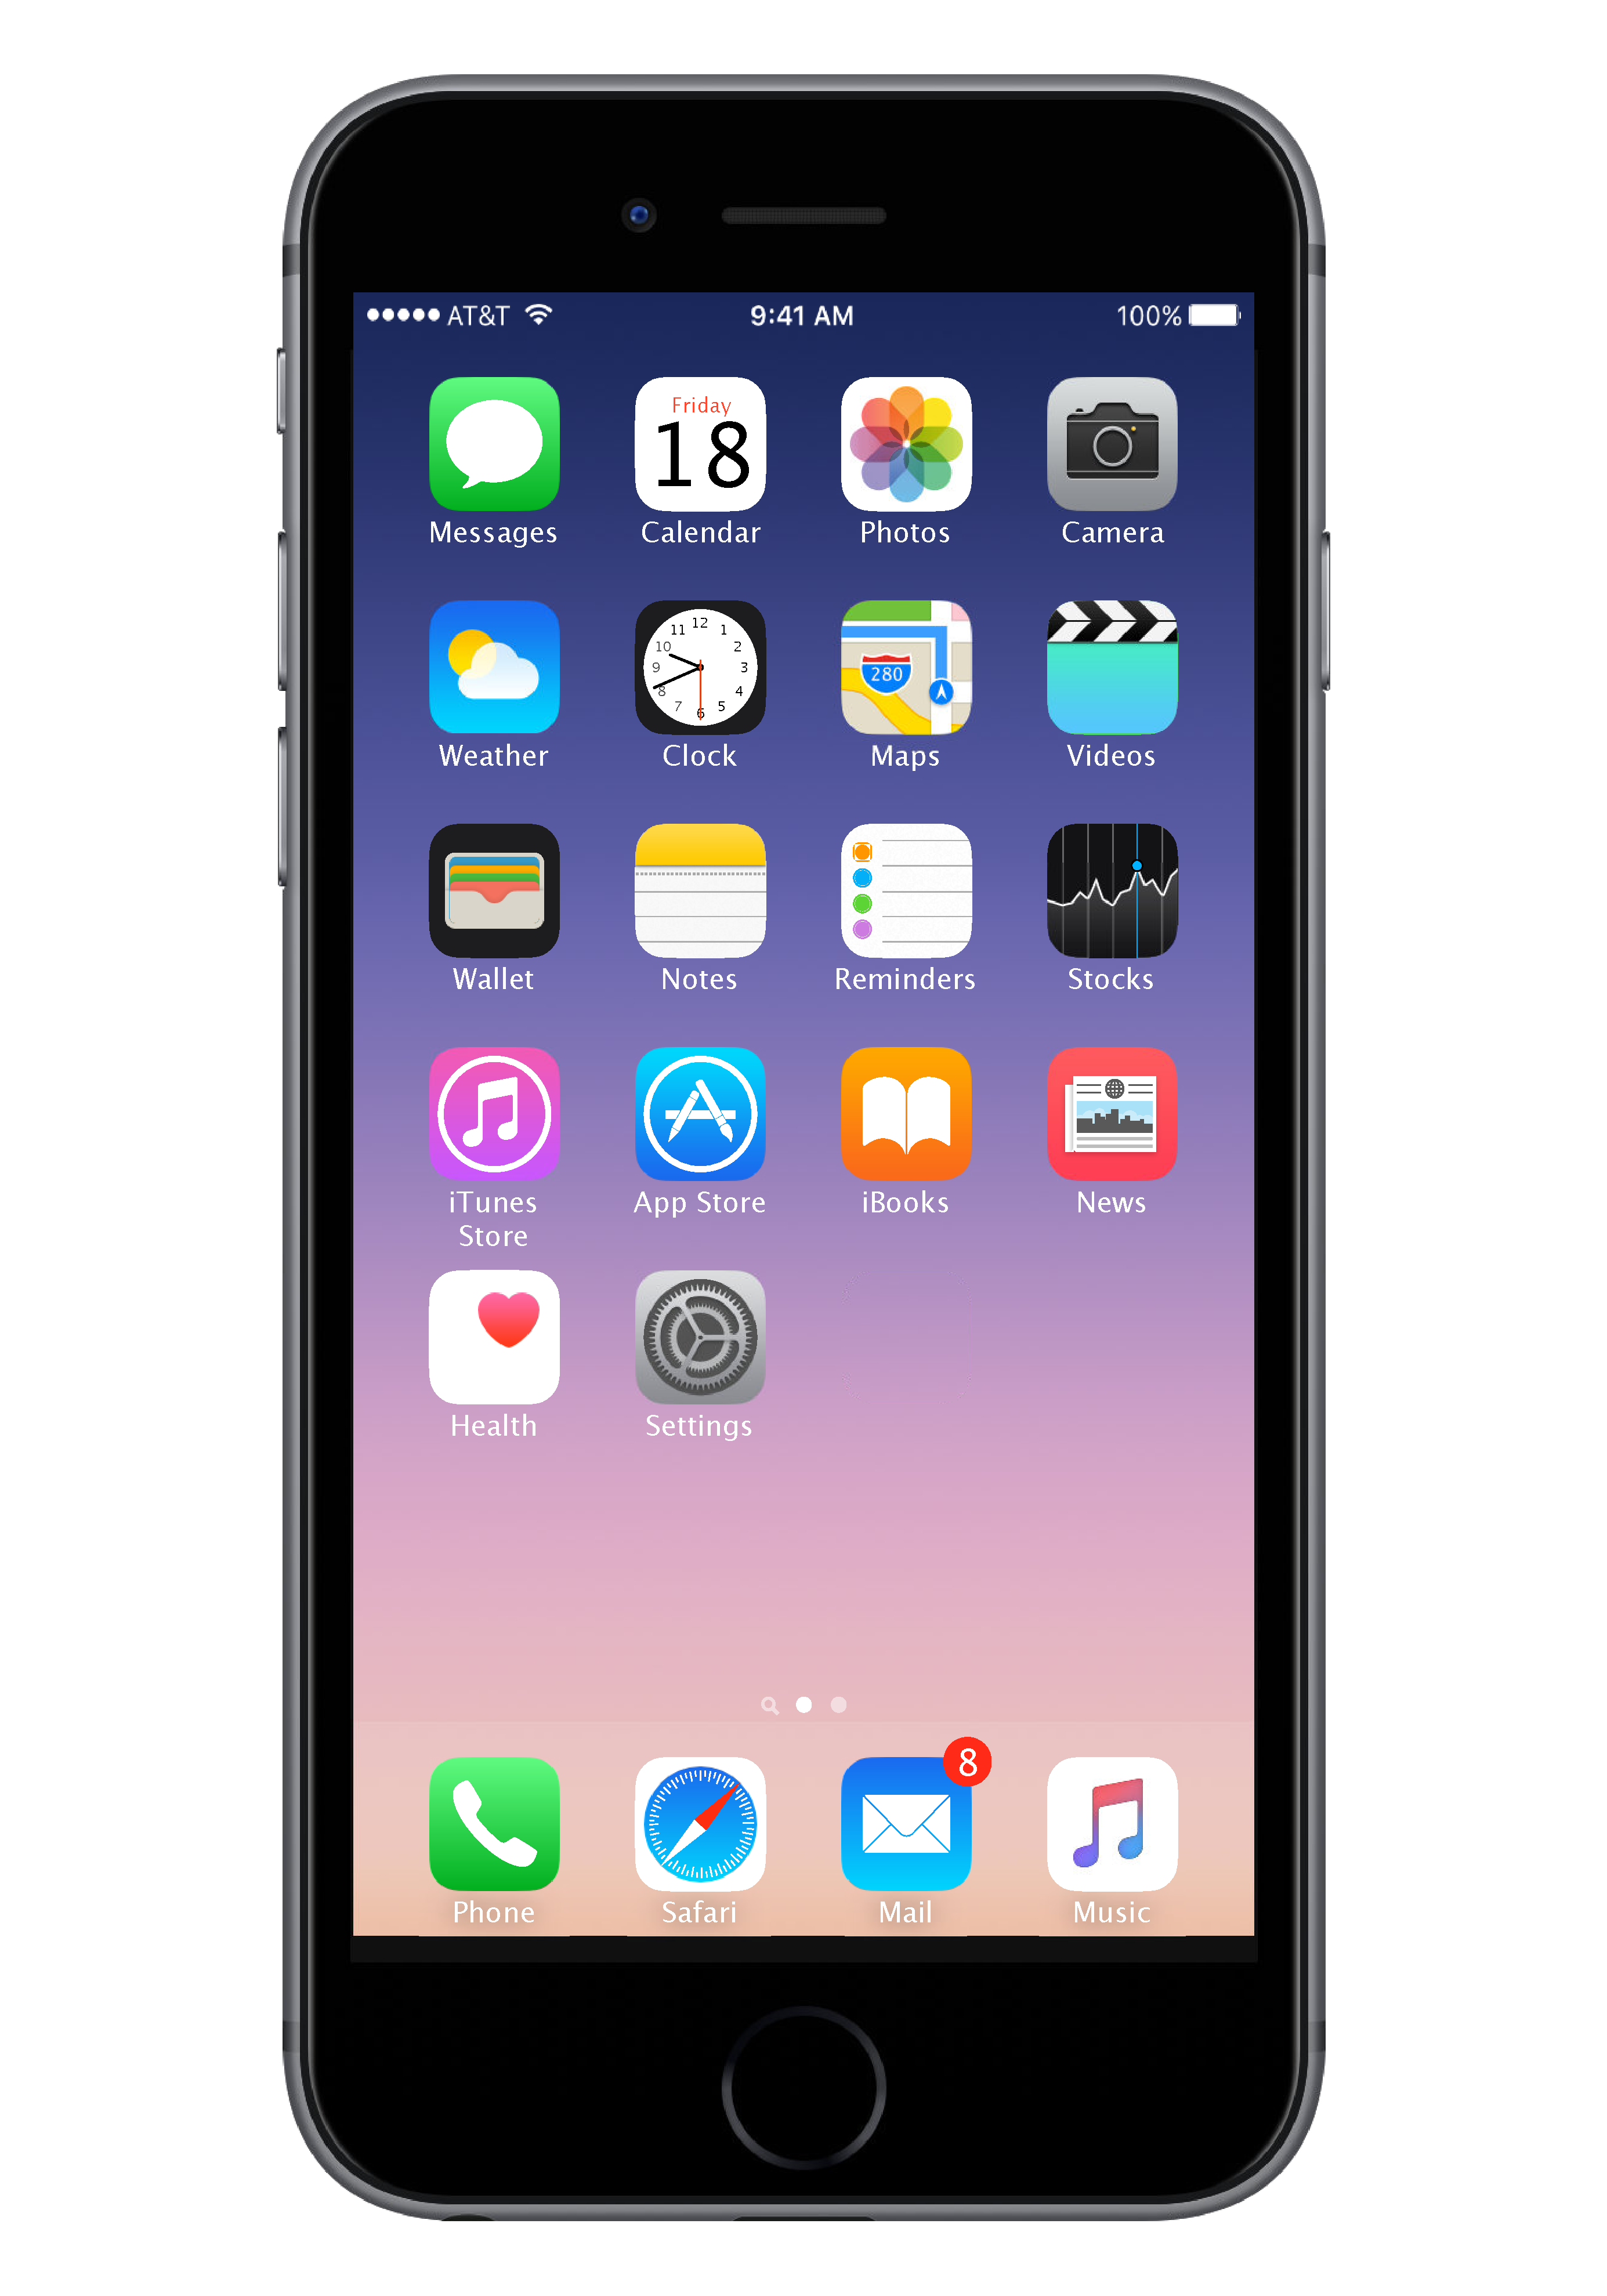
\includegraphics[scale=0.08]
    {textures/images/mac/historic/iOS.pdf}
    \caption{Système d'exploitation iOS}
  \end{figure}

\newpage

\subsection{Popularité}
Les avis à l’encontre de Mac OS X sont assez partagés. \\

Par exemple, les détracteurs pointent du doigt le prix fort élevé à l’achat
ainsi que la presque impossibilité de mise à jour matérielle des macs. \\
Par contre, ces personnes sont souvent des personnes n’ayant jamais utilisé de
Mac. Ils ont alors une vision biaisée leur faisant croire que rien n’est gratuit,
ainsi des fonctionnalités comme le \textit{couper-coller} seraient payantes, ou
bien que l’on ne peut pas faire autant de choses que sur d’autres systèmes comme
Windows. \\

Les partisans mettent par contre en avant la stabilité, la sécurité, la fiabilité
et la vitesse de l’OS. \\
Depuis des années, la facilité d’utilisation est une des forces des systèmes d’Apple,
ainsi que sa base UNIX qui offre la puissance de la ligne de commande au système. \\

Ce n’est un secret pour personne, l’augmentation des parts de marché des Macs
est principalement due à la popularité des iPods, puis principalement des iPhones
et des iPads. \\
Un point positif pour toute personne possédant un appareil Apple: les systèmes
étant proches, passer de l’un à un l’autre ne sera pas dépaysant. De plus, avoir
un ou des appareils mobiles et un mac crée un écosystème permettant de gagner du
temps ainsi que des fonctionnalités. \\

Par défaut, OS X possède de nombreuses fonctionnalités et applications
préinstallées. \\
Mais il en existe d’autres disponibles gratuitement comme \textit{Xcode},
l’IDE d’Apple nécessaire pour créer des applications iOS et qui donne accès à
des outils en ligne de commande comme un compilateur C, et \textit{iWork},
la suite bureautique d’Apple disponible aussi sur iOS et au travers de
n’importe quel navigateur web. \\

\clearpage

\subsection{Fonctionnalités}
Pour commencer, Apple a un avantage sur ses concurrents: l'entreprise ne
s'occupe pas seulement du système d'exploitation, mais aussi des ordinateurs
qui l'utilisent: ils sont donc pensés pour fonctionner en adéquation. Grâce à
cela, Apple peut sortir des sentiers battus et exploiter de nouvelles
technologies tandis que les autres constructeurs doivent attendre que l'OS dont
ils dépendent prenne en considération l'utilité de telle ou telle nouveauté. \\

Par exemple, l'utilisation d'un trackpad multitouch permettant l'utilisation de
gestes tactiles sur ordinateur existe depuis des années sur Mac, et arrive
maintenant chez la concurrence. On peut aussi parler du \textit{Thunderbolt} qui
n'est utilisé que par Apple et qui peut connecter jusqu'à 6 périphériques avec
un débit de 10 Gbit/s dans les deux sens. Son utilisation pourrait se démocratiser
avec le changement de connecteur qui passerait du Mini DisplayPort à l'USB-C et
avec le débit qui doublerait. \\

De plus, grâce au fait qu'Apple développe les systèmes d'exploitation et les
appareils qui les utilisent, un utilisateur d'iPhone ne sera pas dépaysé lors
de l'utilisation d'un Mac, et vice-versa. \\
Il est à noter qu'avec la sortie du \textit{Surface Book} de Microsoft,
Apple n'est plus la seule entreprise à proposer des ordinateurs créés en
parallèle de leur système d'exploitation. \\ Cela pourrait donner un avantage
certain à Microsoft par rapport à ses « \textit{concurrents} » sur Windows. \\

Du côté logiciel, il existe certaines fonctionnalités exclusives à Mac OS X:
\\

\begin{itemize}
\item \textbf{Quick Look} : activé avec un geste multitouch ou la barre d'espace,
permet de montrer un aperçu du fichier/dossier sélectionné sans avoir à
l'ouvrir. Sur un mot, il en donne la définition et/ou la traduction; il donnera
un aperçu de la page web si c'est une URL qui est ciblée. \\

\item \textbf{Time Machine} : une fois activé et un disque dur externe
sélectionné, le système sauvegarde tous les fichiers (nouveaux ou mis à jour)
de l'ordinateur par date et heure. Il est alors facile de retrouver des données
perdues. \\

%\newpage

\item \textbf{AirDrop} : il suffit d'avoir deux appareils Apple connectés au
même réseau Wi-Fi et en Bluetooth pour qu'ils puissent s'échanger des fichiers
d'un simple \textit{drag-and-drop}. \\

\item \textbf{Handoff} : il s'agit d'une fonctionnalité découlant directement
de la politique préférant une convergence des OS plutôt qu'une fusion. Elle
consiste à connecter deux appareils comme un iPad et un Mac entre eux, à
condition qu'ils soient sur un même réseau Wi-Fi et connectés en Bluetooth.
L'utilisateur lit un article en ligne sur son Mac et doit partir; il peut alors
ouvrir le même article sur son iPad en un seul clic. \\

\item \textbf{Continuity} (Continuité) : elle regroupe quatre fonctionnalités:
\textit{AirDrop}, \textit{Handoff}, \textit{Instant Hotspot} qui active le
partage de connexion de l'iPhone lorsqu’il est à proximité du Mac et qu'il n'y
a plus de Wi-Fi et \textit{Téléphone et SMS}. \\
 Cette dernière permet de connecter un iPad ou un Mac à un iPhone afin de
recevoir et envoyer des coups de téléphone ou des SMS sans avoir à prendre son
téléphone. \\

\item \textbf{Raccourcis} : sur OS X, les raccourcis systèmes sont tous regroupés
dans les réglages. \\
Pour ajouter un accent sur une lettre, pas besoin d'appuyer sur plusieurs touches:
un appui long sur la lettre affiche tous les accents possibles, il suffit de choisir. \\
En plus de cela, le système permet de créer des abréviations (\textit{'tjrs'
devient 'toujours'}) et corrige l'orthographe automatiquement. \\

\item (\textbf{...}) \\
\end{itemize}

\begin{figure}[!htb] \minipage{0.45\textwidth}
  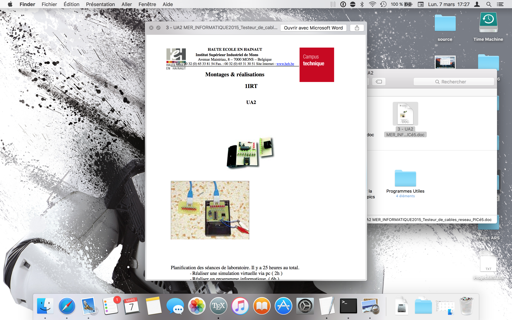
\includegraphics[width=\linewidth]
  {textures/images/mac/features/QuickLook.png}
  \caption{Quick Look}\label{fig: Quick Look}
	\endminipage\hfill \minipage{0.45\textwidth}
  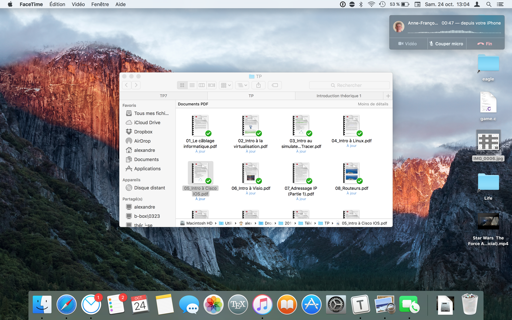
\includegraphics[width=\linewidth]{textures/images/mac/features/Phone.png}
  \caption{Téléphone}\label{fig:Telephone}
	\endminipage
\end{figure}

Pour terminer, Mac OS X ayant un noyau UNIX, l'utilisation du terminal y est à
peu près identique à celle sur Linux. \\
De plus, certains langages de programmation y sont déjà préinstallés comme Java,
Python, Ruby,…

\newpage
\section{Autres systèmes}
\subsection{Précision}
Il existe de nombreux systèmes d'exploitation qui nous sont, en partie,
inconnus. \\

La raison est simple: les systèmes d'exploitation que nous connaissons ont dû se
développer sur base de systèmes d'exploitation expérimentaux qui ne sont plus
utilisés. \\

Exemple : \\

\begin{itemize}
\item Singularity : utilisé pour les recherches de Microsoft; \\

\item MyOS : mini système d'exploitation créé à l'aide du langage C++; \\

\item Desert Spring-Time (\textit{DST}) : système d'exploitation développé en
Objective Caml; \\

\item Kid Operating System (\textit{KOS}) : utilisé pour l'apprentissage; \\

\item (\textbf{...}) \\
\end{itemize}

En outre, il y a des systèmes d'exploitation pour smartphone qui ont été mis de
côté suite à l'abandon de leur développement au profit d'autres technologies. \\

Exemple : \\

\begin{itemize}
\item Symbian : développé par Nokia; \\

\item Meego : développé par Nokia et Intel; \\

\item BlackberryOS : développé par Research In Motion; \\

\item Bada : développé par Samsung; \\

\item (\textbf{...})
\end{itemize}

\newpage

De plus, la majorité des appareils électriques ont un système d'exploitation,
nommé \textit{système embarqué}. \\
C'est lui qui permet de gérer l'aspect informatique du composant; de même, que
d'offrir une interface graphique conviviale à l'utilisateur pour interagir avec
ces appareils. \\

Par exemple, il en existe pour la télévision: \\

\begin{itemize}
\item Tizen : développé par Samsung; \\

\item WebOS : développé par LG; \\

\item tvOS : développé par Apple pour l'Apple TV; \\

\item Android TV : développé par Android; \\

\item (\textbf{...}) \\
\end{itemize}

Les voitures et les camions possèdent un ordinateur intégré qui les contrôle,
comme l'ABS (\textit{système antiblocage des roues}) qui est contrôlé par
l'ordinateur de bord. \\
L'un des plus gros problèmes est la sécurité. \\En effet, si un malandrin pirate
le système d'une voiture, il peut très bien couper le moteur de la voiture au
beau milieu de l'autoroute et le conducteur ne pourra même pas le rallumer ! \\
Ce qu'il faudrait alors, c'est mettre à jour le système, un peu comme pour les
\textit{Teslas} qui reçoivent des mises à jour par Internet, mais le procédé
n'est pas encore assez fiable…

\clearpage

\subsection{Cisco IOS}
Cisco IOS (\textit{Internetwork Operating System}) est le leader mondial des
systèmes d'exploitation de réseau, il est développé par \textit{Cisco Systems}
et équipe la plupart de leurs équipements.

\begin{figure}[!h]
  \centering
  
\includegraphics[scale=0.15]
  {textures/images/others/Cisco_logo.pdf}
  \caption{Logo de Cisco Systems}
\end{figure}

Il est décliné en différentes versions spécialisées pour chaque équipement
(\textit{routeur, commutateur, points d’accès Wi-Fi,…}). \\
L’accès se fait par le port console (ou auxiliaire), Telnet ou SSH, et en ligne
de commande (\textbf{CLI}) ou par une interface web. \\

Du côté de la sécurité, l’accès au périphérique et l’accès au mode d’exécution
privilégié peuvent être protégés par un mot de passe de même. \\

En effet, il existe plusieurs modes d’exécution:

\begin{enumerate}
\item le mode d’exécution utilisateur : point d’entrée de base de la CLI,
  les commandes y sont restreintes;

\item le mode d’exécution privilégié : il permet d’accéder aux informations
  détaillées et aux commandes de configuration et de gestion du périphérique;

\item le mode de configuration globale : permet d’effectuer des commandes de
  configuration globales sur l’équipement;

\item les autres sous-modes : accessibles depuis le mode global, ils permettent
  de configurer des interfaces (\textit{Vlan, VTY, etc.}). \\
\end{enumerate}

Il existe d’autres systèmes d’exploitation de Cisco. \\
Par exemple:

\begin{itemize}
\item CatOS : répandu dans les commutateurs Ethernet haut de gamme, il provient
  de la gamme de commutateurs Catalyst;

\item IOS XE : basé sur Linux, il est compatible avec IOS et est utilisé par les
  entreprises et les fournisseurs de services;

\item NX-OS : pour les commutateurs Ethernet Nexus et les commutateurs à fibre
  optique MDS. Il est basé sur SAN-OS, développé à l'origine pour les commutateurs
  MDS.
\end{itemize}

\newpage
\section{Conclusion}
\label{sec:conclusion}


\subsection{Résultat}
\label{sec:resultat}

L'automate trie les boites d'après leur couleur \textit{(argent, cuivre et or)}.\\

Lorsqu'il est à l'arrêt, la lampe \textit{Hors-service} est allumée, et la lampe \textit{En service} est éteinte. \\

L'appui sur le bouton poussoir  \guillemotleft \ \textbf{Start} \guillemotright \ allume la lampe \textit{En service}, éteint la lampe \textit{Hors-service} et met en route le moteur du convoyeur principal.\\
Sauf dans le cas où un défaut moteur a été détecté, ce qui arrêterait \textit{totalement} le fonctionnement de l'automate.\\
Celui-ci devra d'abord être corrigé afin de désactiver l'alarme lumineuse par un acquittement à l'aide du sélecteur à clé \textbf{I16}. Le moteur pourra alors être mis en route.\\

Pour mettre en marche le moteur des convoyeurs d'évacuation, le sélecteur \textbf{I17} doit être enclenché.\\
S'il n'est pas enclenché, un défaut moteur sera levé et affiché par la lampe \textbf{Q1}. Voici les différents cas qui lèveront le défaut :

\begin{itemize}
    
    \item le cas du défaut au moteur principal, c'est le cas le plus simple.\\
    Le moteur se retrouve en surcharge, ce qui enclenche l'arrêt d'urgence.
    
    \item le cas du défaut au moteur des convoyeurs d'évacuation, divisé en différents cas.
    
    \begin{itemize}
    
        \item le cas simple, le moteur est en surcharge, ce qui enclenche l'arrêt d'urgence.
        
        \item le cas de l'encombrement des tapis d’évacuation.\\
        Il est levé lorsqu'une boite est sous le détecteur du tapis d'évacuation, et qu'une autre \textit{(du même type)} se retrouve devant le vérin.\\
        C'est le cas lorsque le moteur des tapis d’évacuation est à l'arrêt.
        
        \item le cas \textit{bonus}, les tapis d'évacuation sont stoppés, mais le moteur principal ne l'est pas.\\
        Lorsqu'une boite est détectée par le dernier détecteur, \textbf{I3}, un défaut est levé.\\
        Sans ce dernier cas, la boite tomberait du tapis.
        
    \end{itemize}
    
\end{itemize}

\newpage

Lorsqu'une boite argentée ou cuivrée est repérée par le détecteur idoine, le moteur principal s'arrête et le vérin place la boite sur le tapis d'évacuation approprié.\\
Le vérin se replace et le moteur principal se relance une fois que la boite est détectée sur son tapis d'évacuation.\\
À ce moment, le compteur qui lui est lié s'incrémente de un.\\

Pour les boites dorées, il n'y a pas de vérin, donc pas d'arrêt du moteur principal.\\
En effet, une fois arrivées au bout du tapis principal, les boites se retrouvent sur le tapis d'évacuation correct s'il est activé.\\
C'est alors le dernier détecteur, \textbf{I3}, qui incrémente le compteur adéquat.\\

Les compteurs sont réinitialisés dans deux cas :

\begin{itemize}
    
    \item premier cas, l'automate est stoppé par le bouton poussoir \guillemotleft \ \textbf{Stop} \guillemotright.
    
    \item second et dernier cas, le sélecteur à clé, \textbf{I18}, est activé afin de réinitialiser les compteurs à la main.
    
\end{itemize}

\newpage
\nocite{*}
\addcontentsline{toc}{section}{Références}

\begin{category}{Livres}
    \SBentries{algo}
    \SBentries{cHeH}
    \SBentries{csHeH}
    \SBentries{cZero}
    \SBentries{javaZero}
    \SBentries{latex}
    \SBentries{mor}
\end{category}

\begin{category}{Internet}
    \SBentries{website:bootstrap}
    \SBentries{website:laravel}
    \SBentries{website:pythonWiki}
    \SBentries{website:pythonZero}
    \SBentries{website:slider}
    \SBentries{website:xDupre}
\end{category}

\bibliographystyle{acm} 
\bibliography{bibli}


\newpage
\section*{Figures}
\addcontentsline{toc}{section}{Figures}

[1, 2, 29, 31, 32] Images personnelles \\

[3, 4, 5, 6, 7, 14, 15, 16, 17, 18, 19] \href{https://commons.wikimedia.org}{https://commons.wikimedia.org} \\

[8] \href{https://tecnoblog.net/wp-content/uploads/2015/10/windows-1-de-volta-futuro.png}
{https://tecnoblog.net} \\

[9] \href{https://cdn0.vox-cdn.com/thumbor/xw68yMxmzret66x1Eb2h4YpnvRw=/cdn0.vox-cdn.com/uploads/chorus_asset/file/3913062/Screenshot__40_.0.png}
{https://cdn0.vox-cdn.com} \\

[10] \href{http://az648995.vo.msecnd.net/win/2015/01/phone_start.png}
{http://az648995.vo.msecnd.net/win/2015/01/phone\_start.png} \\

[11] \href{http://www.ariase.com/fr/news/media/windows10-04.jpg}
{http://www.ariase.com/fr/news/media/windows10-04.jpg} \\

[12] \href{http://az648995.vo.msecnd.net/win/2015/03/Gallo-blog-1-v2.png}
{http://az648995.vo.msecnd.net/win/2015/03/Gallo-blog-1-v2.png} \\

[13] \href{http:/umons.ac.be}{http:/umons.ac.be} \\

[20] \href{https://doc.ubuntu-fr.org/lib/exe/fetch.php?tok=c9ce59\&media=http\%3A\%2F\%2Fpix.toile-libre.org\%2Fupload\%2Foriginal\%2F1337006028.png}
{https://doc.ubuntu-fr.org} \\

[21] \href{https://upload.wikimedia.org/wikipedia/commons/9/97/GNOME_Shell.png}
{https://upload.wikimedia.org/wikipedia/commons/9/97/GNOME\_Shell.png} \\

[22] \href{https://upload.wikimedia.org/wikipedia/commons/9/97/Kubuntu-12.10-desktop.png}
{https://upload.wikimedia.org/wikipedia/commons/9/97/Kubuntu-desktop.png} \\

[23] \href{http://2.bp.blogspot.com/-F26Pbg1pDuc/UH-l-hoBvDI/AAAAAAAAK-c/NuK3Hhp0B4c/s1600/xubuntu12.10.png}
{http://2.bp.blogspot.com} \\

[24] \href{http://consumer.huawei.com/minisite/worldwide/nexus6p/assets/nexus/images/nexus-intro-phone-1.png}
{http://consumer.huawei.com} \\

[25] \href{http://drop.ndtv.com/TECH/product_database/images/2182016105729AM_635_meizu_pro_5_ubuntu_edition.jpeg}
{http://drop.ndtv.com} \\

[26] \href{http://www.guidebookgallery.org/screenshots/apple2desktop11}
{http://www.guidebookgallery.org/screenshots/apple2desktop11} \\

[27] \href{http://apple.wikia.com/wiki/System_1}
{http://apple.wikia.com/wiki/System\_1} \\

[28] \href{http://winmac.emuunlim.com/SSFrame.html}
{http://winmac.emuunlim.com/SSFrame.html} \\

[30] \href{http://ozzik.co/freebies/ios9kit}
{http://ozzik.co/freebies/ios9kit} \\

[33] \href{https://commons.wikimedia.org/wiki/File:Cisco_logo.svg}
{https://commons.wikimedia.org/wiki/File:Cisco\_logo.svg} \\

\newpage
\section*{Questionnaire}
\addcontentsline{toc}{section}{Questionnaire}

\begin{enumerate}
  \item Guillaume est dubitatif lors de la lecture d’un site sur lequel est écrit: \\
  « La ligne de commande est apparue pour faciliter le dialogue entre les OS
  et les utilisateurs, vu que l’interface graphique n’était pas assez
  puissante ». \\
  Le Webmaster a-t-il raison ? \textbf{Faux} \\

  Depuis les années 80, l’interface graphique est utilisée à la place de
  l’interface en ligne de commande, car elle ne nécessite pas l'apprentissage
  de commandes pour utiliser un ordinateur.\\
  Par contre, sur les systèmes dérivés d’UNIX, la ligne de commande reste
  fortement utilisée étant donné la richesse des possibilités. \\

  \item D’après Gino, plus de 90 \% des 500 ordinateurs les plus puissants au monde
  et des serveurs seraient équipés de Linux. \\
  Est-ce bien vrai ? \textbf{Vrai}\\

  En effet, Linux tourne sur 98 \% des serveurs Web mondiaux et \\
  sur 92 \% des 500 supercalculateurs les plus puissants. \\

  \item Lors d’une présentation, Alexandre annonce que les systèmes d’exploitation
  d’Apple sont basés sur Ubuntu, mais cette affirmation ne fait pas
  l’unanimité. \\
  A-t-il raison ? \textbf{Faux} \\

  Mac OS X et ses dérivés sont basés sur \textit{NeXTSTEP} qui l'était lui-même
  sur l’implémentation BSD d’UNIX. \\
  Ubuntu est basé sur \textit{Debian} qui est un UNIX-like. \\

  \item Un site affirme que la version de Windows 10 pour tablettes est identique à
  celle pour smartphones, mais Antoine n’y croit pas. \\
  Le site a-t-il raison ? \textbf{Faux} \\

  Le système d'exploitation des \textit{Surfaces} de Microsoft est Windows 10,
  alors que les Windows Phones utilisent un système adapté: Windows 10 Mobile. \\

  \clearpage

  \item Lors de son entrevue avec les policiers, Julien soutient que sa voiture a
  été piratée sur l’autoroute avant qu’elle ne s’éteigne d’un coup. \\
  Est-ce possible ? \textbf{Vrai} \\

  Les voitures étant contrôlées par un ordinateur de bord, il suffit que la
  voiture soit connectée à Internet pour qu'un hacker la pirate. \\
  Une fois piratée, il peut très bien arrêter le moteur, bloquer les freins ou
  même prendre la main sur le volant ! \\
  Tout cela à distance, bien entendu. \\

  \item Sarah a installé Ubuntu en Dual Boot avec Windows. Après avoir installé des
  logiciels téléchargés depuis Linux, sa session Windows est infectée par un
  virus. \\
  Est-ce possible d’attraper un virus depuis Linux ? \textbf{Vrai} \\

  Il est en effet possible de télécharger des virus pour n'importe quel OS
  depuis Internet. Une fois le virus téléchargé, l'ordinateur devient un
  porteur sain si le virus n'est pas prévu pour ce système. \\
  Il est donc concevable qu'un fichier inoffensif sur Linux soit transféré sur
  un autre OS qui, lui, devienne infecté. \\
  C'est pour cela qu'il est important d'avoir un pare-feu, antivirus
  (\textit{qui bloquera les virus pour tous les OS}), ... \\

  \item Lors d’un labo d’électronique, Thibault demande à Alexandre de lui envoyer
  une photo de son circuit. \\
  Ayant tous deux un iPhone, ils se l’échangent grâce à Quick Look. \\
  Ont-ils utilisé la bonne fonctionnalité ? \textbf{Faux} \\

  Quick Look permet de montrer l’aperçu d’un fichier, dossier ou site ou la
  définition d’un mot. \\
  Pour le partage de fichiers, c’est AirDrop qui est utilisé, à condition
  d’activer le Bluetooth et d’être sur le même réseau Wi-Fi. \\

  \clearpage

  \item Lorsqu’il se relit, Clément pense s’être trompé en notant que « un
  environnement de bureau est un ensemble de logiciels et d’un système
  d’exploitation, comme Ubuntu et Red Hat ». \\
  Cette note est-elle correcte ? \textbf{Faux} \\

  Cette définition est celle d'une distribution. \\
  Un environnement de bureau, lui, constitue les caractéristiques graphiques
  du système d’exploitation et permet à l’utilisateur d’interagir avec son
  ordinateur. \\
  C'est lui qui gère les fenêtres, le bureau, etc. \\

  \item Lorenzo ne croit pas qu’Android est basé sur Linux et qu’il peut être
  utilisé sur ordinateur. \\
  L’information est-elle correcte ? \textbf{Vrai} \\

  Android est basé sur un noyau Linux. \\
  Initialement disponible uniquement sur smartphones, Android s'est décliné sur
  tablettes, télévisions, consoles de jeux et montres connectées. \\
  Depuis 2011, Android-x86 est disponible pour les ordinateurs possédant un
  processeur x86 et x64 de Intel. \\

  \item Arnaud ne croit pas qu’un OS a deux fonctions majeures: la gestion des
  ressources matérielles et la fourniture de services aux applications. \\
  Thomas lui rétorque qu’il se trompe, mais est-ce vrai ? \textbf{Vrai} \\

  En effet, un système d'exploitation a deux fonctions majeures. \\
  Si une application requiert des informations, c'est à lui qu'elle fait appel. \\
  Elle s'occupe aussi du démarrage, de la gestion du processeur et de la
  mémoire. \\

  \item Avant de l’appeler iOS, Steve Jobs l’a nommé \textit{idealOS} vu qu’il était \\
  « le système d’exploitation idéal pour l’iPhone ». \\
  Cette information venant de Wikipédia est-elle véridique ? \textbf{Faux} \\

  C'était le système d'exploitation des iPhones ainsi que des iPod Touch.
  Il était alors appelé \textit{iPhoneOS}. \\
  En 2010, il devient iOS avec la sortie de l'iPad. \\

  \item Lors d’une présentation, Laurent entend cette affirmation : les OS ont de
  nombreux rôles comme la gestion des droits, de la sécurité ainsi que
  l’exécution des logiciels. \\
  Est-elle vraie ? \textbf{Vrai} \\

  Un système d'exploitation a de nombreux rôles dont la gestion des droits, de
  la sécurité et l’exécution des logiciels. \\
  Cependant, on peut rajouter la gestion du processeur, de la mémoire ainsi que des
  environnements de bureaux. \\

  \item Pendant son stage, Anthony a appris, avec scepticisme, que Cisco IOS était
  basé sur Linux. \\
  Après quelques recherches, il est fixé, mais était-ce vrai ? \textbf{Faux} \\

  Cisco IOS n'est pas lié à Linux: c'est un système développé entièrement par
  Cisco Systems. \\
  Par contre, Cisco IOS XE (ou IOS XE) est bien basé sur Linux et est
  entièrement compatible avec Cisco IOS. \\

  \item Florian prétend qu’il peut déverrouiller son ordinateur sous Windows avec
  ses yeux, ses amis ne le croient pas. \\
  Dit-il la vérité ? \textbf{Vrai} \\

  Windows 10 intègre Windows Hello, qui permet de déverrouiller sa session avec
  son visage, son iris ou son doigt à condition de posséder un périphérique
  compatible. \\

  \item D’après les dires de Burak, il est tout à fait possible d’utiliser Windows
  10 Mobile comme on le fait avec un ordinateur. \\
  Est-ce vrai ? \textbf{Vrai… et Faux} \\

  Grâce à une station d'accueil dédiée, on peut utiliser son smartphone sous
  Windows 10 Mobile sur un grand écran avec un clavier et une souris. \\
  Mais ce n'est que Windows Mobile, il ne peut pas faire autant qu'un
  ordinateur: moins de fonctionnalités, pas de multitâche, etc.

\end{enumerate}

\newpage
\newpage
\thispagestyle{empty}
\setcounter{page}{0}
\null
\newpage
\end{document}
